\documentclass{tufte-handout} % A4 paper and 11pt font size
\usepackage[activate={true,nocompatibility},final,tracking=true,kerning=true,spacing=true,factor=1100,stretch=10,shrink=10]{microtype}
\usepackage[T1]{fontenc} % Use 8-bit encoding that has 256 glyphs
%\usepackage{mathpazo} % Use the Adobe Utopia font for the document - comment this line to return to the LaTeX default
\usepackage[english, serbianc]{babel} % English language/hyphenation
\usepackage{amsmath,amsfonts,amsthm, amssymb} % Math packages
\usepackage{pgf,tikz}
\usetikzlibrary{positioning,matrix,arrows}
\usepackage{float}
\usepackage{tikz-cd}
\usepackage{caption}
\usepackage{stmaryrd}
\usepackage{multicol}
\usepackage{booktabs}
\usepackage{verbatim}
\usepackage{lipsum} % Used for inserting dummy 'Lorem ipsum' text into the template
\usepackage{sectsty} % Allows customizing section commands
\usepackage{titlesec}
\usepackage{empheq}
\usepackage[most]{tcolorbox}
\usepackage{hyperref}
%Boxed eqns
\newcommand{\boxedeq}[1]{\begin{empheq}[box={\fboxsep=6pt\fbox}]{align} #1\end{empheq}}

\allsectionsfont{\normalfont \bfseries} % Make all sections centered, the default font and small caps
\usepackage{enumerate}
\usepackage{pythonhighlight}
\usepackage{fancyhdr} % Custom headers and footers
\pagestyle{fancyplain} % Makes all pages in the document conform to the custom headers and footers
\fancyhead{} % No page header - if you want one, create it in the same way as the footers below
\fancyfoot[L]{} % Empty left footer
\fancyfoot[C]{} % Empty center footer
\fancyfoot[R]{\thepage} % Page numbering for right footer
\renewcommand{\headrulewidth}{0pt} % Remove header underlines
\renewcommand{\footrulewidth}{0pt} % Remove footer underlines
\setlength{\headheight}{13.6pt} % Customize the height of the header
\allowdisplaybreaks

\usepackage{wrapfig}
\graphicspath{ {./slike/} }

%Sections

%--------Theorem Environments--------
%theoremstyle{plain} --- default
\newtheorem{thm}{Theorem}
\newtheorem{cor}[thm]{Corollary}
\newtheorem{prop}[thm]{Proposition}
\newtheorem{facts}[thm]{Facts}
\newtheorem{fact}[thm]{Fact}
\newtheorem{clm}[thm]{Claim}
\newtheorem{lem}[thm]{Lemma}
\newtheorem{conj}[thm]{Conjecture}
\newtheorem{quest}[thm]{Question}

\theoremstyle{definition}
\newtheorem{defn}[thm]{Definition}
\newtheorem{defns}[thm]{Definitions}
\newtheorem{con}[thm]{Construction}
\newtheorem{exmp}[thm]{Example}
\newtheorem{exmps}[thm]{Examples}
\newtheorem{notn}[thm]{Notation}
\newtheorem{notns}[thm]{Notations}
\newtheorem{addm}[thm]{Addendum}
\newtheorem{exer}[thm]{Exercise}

\theoremstyle{remark}
\newtheorem{rem}[thm]{Remark}
\newtheorem{rems}[thm]{Remarks}
\newtheorem{warn}[thm]{Warning}
\newtheorem{sch}[thm]{Scholium}

\newcommand{\bra}[1]{\left(#1\right)}
\newcommand{\sbra}[1]{\left[#1\right]}
\newcommand{\Mod}[1]{\ (\text{mod}\ #1)}
\newcommand{\op}[1]{#1^{\text{op}}}
\newcommand{\R}{\mathbb{R}}
\newcommand{\N}{\mathbb{N}}
\newcommand{\Z}{\mathbb{Z}}
\newcommand{\mZ}{\mathcal{Z}}
\renewcommand{\C}{\mathbb{C}}
\newcommand{\Q}{\mathbb{Q}}
\newcommand{\F}{\mathbb{F}}
\newcommand{\bA}{\mathbb{A}}
\newcommand{\bH}{\mathbb{H}}
\newcommand{\one}{\mathbb{1}}
\newcommand{\mC}{\mathcal{C}}
\newcommand{\mO}{\mathcal{O}}
\newcommand{\mR}{\mathcal{R}}
\newcommand{\mS}{\mathcal{S}}
\newcommand{\lp}{{\mathfrak{p}}}
\renewcommand{\P}{\mathbb{P}}
\newcommand{\E}{\mathbb{E}}
\DeclareMathOperator{\dist}{dist}
\DeclareMathOperator{\aut}{Aut}
\DeclareMathOperator{\gal}{Gal}
\DeclareMathOperator{\var}{\textbf{var}}
\DeclareMathOperator{\orb}{Orb}
\DeclareMathOperator{\ff}{Frac}
\DeclareMathOperator{\stab}{Stab}
\DeclareMathOperator{\inn}{Inn}
\DeclareMathOperator{\Ind}{Ind}
\DeclareMathOperator{\Res}{Res}
\DeclareMathOperator{\spn}{Span}
\DeclareMathOperator{\out}{Out}
\DeclareMathOperator{\im}{Im}
\DeclareMathOperator{\rk}{rk}
\DeclareMathOperator{\disc}{disc}
\DeclareMathOperator{\tors}{Tors}
\DeclareMathOperator{\Mor}{Mor}
\DeclareMathOperator{\End}{End}
\DeclareMathOperator{\Hom}{Hom}
\DeclareMathOperator{\Nat}{Nat}
\DeclareMathOperator{\spec}{Spec}
\DeclareMathOperator{\ann}{Ann}
\DeclareMathOperator{\ord}{ord}
\DeclareMathOperator{\conjc}{Conj}
\DeclareMathOperator{\Br}{Br}
\DeclareMathOperator{\Tr}{Tr}
\DeclareMathOperator{\Nm}{Nm}
\DeclareMathOperator{\Char}{char}
\newcommand{\norm}[1]{\left\lVert #1 \right\rVert}
\newcommand{\inp}[2]{\left\langle #1, #2 \right\rangle}
\newcommand{\shreq}[2]{-\frac{\hbar^2}{2m}\frac{\partial^2 #1}{\partial #2^2} + U(#2) #1 =E #1}
\newcommand{\tshreq}[2]{i\hbar\frac{\partial #1}{\partial t^2} = -\frac{\hbar^2}{2m}\frac{\partial^2 #1}{\partial #2^2} + U(#2) #1}
\newcommand{\kpsi}{\psi^{''}+k\psi=0}
\def \v {\vspace{0.2cm}}

\geometry{
	left=13mm, % left margin
	textwidth=130mm, % main text block
	marginparsep=8mm, % gutter between main text block and margin notes
	marginparwidth=55mm % width of margin notes
}
\fontsize{10}{20}\selectfont
%----------------------------------------------------------------------------------------
%	TITLE SECTION
%----------------------------------------------------------------------------------------

\title{	
	\normalfont\normalsize 
	{Електротехнички факултет, Универзитет у Београду - Летњи семестар 2023.} \\ [0pt] % Your university, school and/or department name(s)
	\huge Белешке - Квантна Механика% The assignment title
}\author{Михаило Стојковић} % Your name
\date{\vspace{-5pt}\normalsize\today} % Today's date or a custom date


\titleformat{\section}
	{}{\noindent\rule{\textwidth}{0.5pt}\\thesection\\\noindent\rule{\textwidth}{0.5pt} }{1em}{}[{\titlerule[0.8pt]}]




\begin{document}
\justifying 
\maketitle

\tableofcontents
\newpage
\vspace{1em}
\hrule
\section{Предавање - 8.3.2023.}
\hrule
\vspace{1em}
Само предавање креће са тим да посматрамо стационарну Шредингерову једначину:
	\boxedeq{\shreq{\psi}{x}}
али у случају када је $U(x)=0$. Заменом $k^2\equiv\frac{2mE}{\hbar^2}$ у претходну једначину\footnote{Оваква смена се често појављује у курсу тако да после неког времена постане стандардно да када год се појави неко $k$ сматрамо да је једнако наведеном изразу} добијамо диференцијалну једначину:
	\boxedeq{\label{eqn:sred_k}\kpsi}
Решење ове диференцијалне једначине можемо изразити у два облика:
\begin{enumerate}
	\item Као збир експоненцијала\footnote{Овај облик решења је јако користан у ситуацијама где нам се Шредингерова једначина сведе на облик сличан једначини (\ref{eqn:sred_k}), где ако је испред коефицијента уз $\psi$ знак минус, функција ће бити чисто реална. Решења у овом облику се често узимају у ситуацијама где разматрамо константну потенцијалну енергију или честицу која се налази у коначној баријери}: $\psi(x)=Ae^{ikx} + Be^{-ikx}$
	\item Као збир синуса и косинуса\footnote{Овај облик решења је јако користан ако на интервалу решавања имамо неку бесконачну баријеру}: $\psi(x)=C\sin(kx)+D\cos(kx)$
\end{enumerate}
Оба облика су решење дате диференцијалне једначине и може се лако показати како једно можемо представити преко другог.\par
Посматрамо решење у експоненцијалном облику. Због хомогености диференцијалне једначине, негативно и позитивно решење можемо посматрати као два засебна решења са додатом функцијом времена.
\begin{align}
	\label{eqn:talas_u_desno}\psi_1(x,t)&=A_1e^{i(kx-\omega t)}\\
	\label{eqn:talas_u_levo}\psi_2(x,t)&=B_1e^{-i(kx-\omega t)} 
\end{align}
и заправо, једначина (\ref{eqn:talas_u_desno}) представља талас који се креће на десно, а једначина (\ref{eqn:talas_u_levo}) представља талас који се креће на лево.

\begin{wrapfigure}{L}{0.5\textwidth}
	\centering
	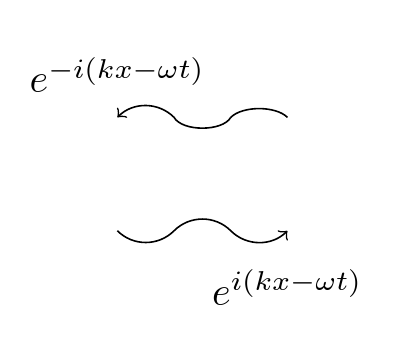
\includegraphics[width=0.5\textwidth]{kretanje_talasa.png}
	\caption{Кретање таласа}
\end{wrapfigure}
Питање које се увек поставља при добитку неког решења једначине: "Да ли ово може представљати таласну једначину". Услови који морају бити испуњени за таласну функцију на неком интервалу су следећи:
\begin{enumerate}
	\item Таласна функција мора бити нормирана\footnote{Погледати (\hyperref[sec:uslov_normiranosti]{Услов нормираности})}
	\item Таласна функција мора бити непрекидна
	\item Први извод таласна функције мора бити непрекидан
\end{enumerate}
При почетку решавања проблема нисмо експлицитно специфицирали интервал решавања, тако да сматрамо да је интервал цело поље $\R$. Овде настаје сада проблем јер решење које смо добили не може да се нормира.
\begin{align}
	\int_{-\infty}^{+\infty}\psi_1^{\ast}\psi_1 dx = |A_1|^2\int_{-\infty}^{+\infty}dx\nless \infty\\ 
	\int_{-\infty}^{+\infty}\psi_2^{\ast}\psi_2 dx = |B_1|^2\int_{-\infty}^{+\infty}dx\nless \infty
\end{align}

Начин на који ово решавамо је мало шкакљив. Претпоставимо да потенцијална енергија није свуда нула, већ само на интервалу $(-\frac{L}{2},\frac{L}{2})$. Ван тог интервала сматрамо да је потенцијална енергија бесконачна, то јест, да честица сигурно мора да се налази на овом интервалу. Ван овог интервала $\psi(x,t)=0$. Бирамо сада функцију (\ref{eqn:talas_u_desno}), без додате функције времена и проверавамо да ли сада можемо да је нормирамо.

\begin{align*}
	&\displaystyle\int_{-\infty}^{+\infty}|\psi_1|^2dx =1\\
	&\displaystyle|A_1|^2\int_{-\frac{L}{2}}^{\frac{L}{2}}|e^{ikx}|^2dx= 1\\
	&|A_1|^2 \cdot L = 1 \implies A_1 = \frac{1}{\sqrt{L}}
\end{align*}
\begin{wrapfigure}{l}{0.5\textwidth}
	\centering
	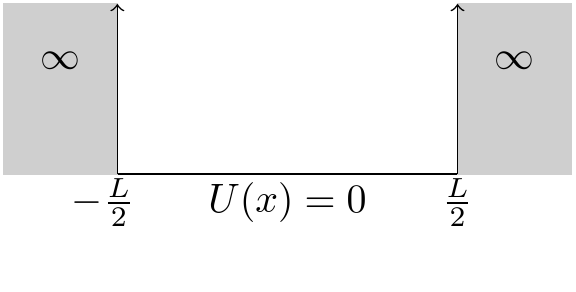
\includegraphics[width=0.5\textwidth]{beskonacne_barijere.png}
	\caption{График потенцијалних баријера. У интервалу $\left(-\frac{L}{2}, \frac{L}{2}\right)$ потенцијална енергија је једнака 0. Ван тог интервала потенцијална енергија је једнака $\infty$}
\end{wrapfigure}
Овим смо добили константу нормирања. Истим поступком можемо добити $B_1$ за једначину (\ref{eqn:talas_u_levo}) и испоставиће се да је једнака $A_1$. Тако да сада имамо решења функција у облику:
\begin{align}
		\psi_1(x)&=\frac{1}{\sqrt{L}}e^{ikx}\\
		\psi_2(x)&=\frac{1}{\sqrt{L}}e^{-ikx} 
\end{align}
Наравно, како би повратили наш првобитни случај, захтевамо да $L\rightarrow\infty$. 

Како би проблем у потпуности решили, морамо да сазнамо какав је спектар енергија. Услов који постављамо за проблеме овог типа(проблеми где уводимо фиктивне границе које теже бесконачности) је да сама функција има исте вредности на оба краја граница.
\begin{align*}
	&\psi_1\left(\frac{L}{2}\right)=\psi_1\left(-\frac{L}{2}\right)\\
	&e^{ik\frac{L}{2}}=e^{-ik\frac{L}{2}}\\
	&e^{ikL}=1
\end{align*}
\begin{figure}[h!]
	\centering
	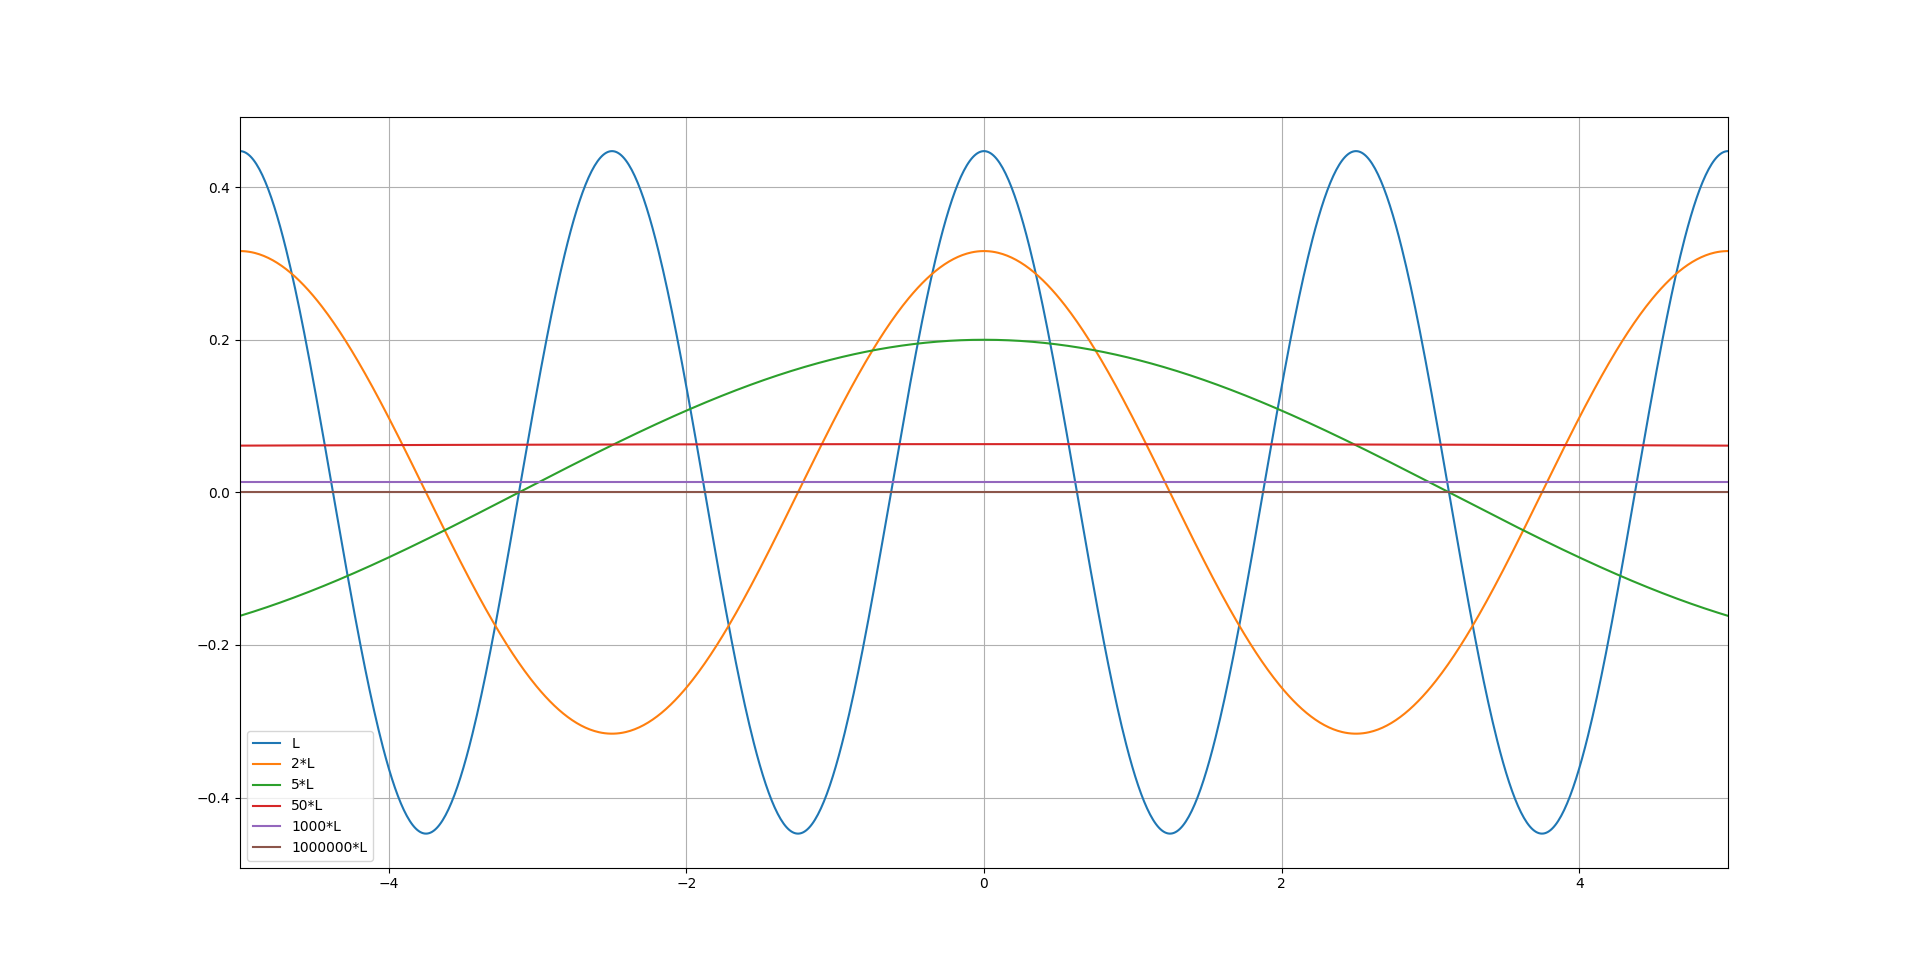
\includegraphics[width=1\textwidth]{grafik_kosinus.png}
	\caption{Графички приказ реалног дела таласне функције $\psi(x)=\frac{1}{\sqrt{L}}e^{ikx}$ са повећањем границе $L$}
\end{figure}
Из последње релације можемо да одредимо вредност $k$ и самим тим и вредност $E$. Овде је битно назначити главни детаљ код оваквих проблема: Увођењем граница довели смо до тога да је спектар дискретан. Једино у граничном случају када баријере теже бесконачности ће се спектар "претворити" у континуалан. Из овога такође закључујемо да проблеми овог типа (без граница) поседују континуални спектар.\par
Додатан детаљ: Ако покушамо да наћемо исти услов за талас који се креће у лево, добићемо идентичну релацију. Одатле закључујемо да у оваквом континуалном спектру постоје две таласне функције које одговарају истој енергији. Број таласних функција у континуалном домену спектра које одговарају истој вредности енергије се назива дегенерација спектра\footnote{У случају који смо разматрали, имамо двоструко дегенерисани континуални спектар}.
\vspace{3em}
\hrule
\subsection*{Слободна честица на полубесконачном домену}
\hrule
\vspace{1em}
\section{Предавање - 10.3.2023.}
\section{Предавање - 22.3.2023.}
\section{Предавање - 24.3.2023.}
\section{Предавање - 29.3.2023.}
\section{Предавање - 5.4.2023.}
\section{Предавање - 7.4.2023.}
\section{Предавање - 12.4.2023.}





\appendix
\section{Услов нормираности}\label{sec:uslov_normiranosti}
Услов нормираности се своди на услов да je функција $f$ на задатом интервалу $(a,b)$ квадратно интеграбилна: \begin{equation*}
	\int_{a}^{b}|f|^2dx<\infty
\end{equation*}
и да је на целом пољу $\R$ једнака 1. То произилази из Копенхагенове интерпретације квантне механике: "\textit{$|\psi|^2dx$ представља вероватноћу да се честица налази у домену $dx$, тако да честица се сигурно налази негде на целом простору}". 
С обзиром да је Шредингерова једначина хомогена, решење ће нам увек бити нека функција $g$ поможена са неком константном $А$ тако да када одредимо интеграл од $|g|^2$, рецимо да је вредност интеграла $I$, потребно је само да поставимо $А=\frac{1}{\sqrt{I}}$. Прецизније, константа је одређена на овај начин до неког мултипликативног фактора $e^{i\alpha}$, где је $\alpha$ неки реалан број. Овај фактор се занемарује јер, иако то мења облик таласне функције са математичког аспекта, физички смисао остаје исти, јер ће при поновном нормирању да се изгуби. Због претходне дискусије увек узимамо да је $А$ реална позитивна константа.

\end{document}